\documentclass[]{article}
\newcommand{\FileDepth}{../..}
\usepackage[a4paper, total={15cm,23cm}]{geometry}
\usepackage[T1]{fontenc}
\usepackage{textcomp}%Not strictly necessary, but gives \textmu command for "micro."
\usepackage{fancyhdr}
\usepackage{amsmath}
\usepackage{amssymb}
\usepackage{graphicx}
\usepackage{xcolor}
\usepackage{tikz}
\usetikzlibrary{calc}
\usepackage{cancel}
%opening
\newcommand{\SecType}{X}
\newcommand{\Week}{X}
\title{Colliding Rocks}
\author{Benjamin Bauml}
\date{Spring 2024}
\pagestyle{fancy}
\rhead{PH 211}
\chead{Spring 2024}
\lhead{Week \Week}

% For Assignment, leave Purpose as 1. For Worksheet, set to 2. For Student Solution, set to 3. For Teacher Solution, set to 4.
% If you want keep the pieces from being called manually, set DefOnly to 0.
\newcommand{\Purpose}{4}
\newcommand{\DefOnly}{1}

% Version 2024-04-27
% Changes
% 2024-02-21 Added xstring package to enable smooth implementation of new \ModePage command.
% 2024-04-27 Set up to split activities and formatting aspects into separate files. Removed dependence on xcomment. Added an automatic counter to number the activities in a problem set.
% 2024-05-19 Revised old format for \TeachingTips command, which did not support \DefOnly.
\usepackage{tcolorbox}
\usepackage{xstring}
% You will want the following four lines in your document (the last two uncommented):
% For Assignment, leave Purpose as 1. For Worksheet, set to 2. For Student Solution, set to 3. For Teacher Solution, set to 4.
% If you want keep the pieces from being called manually, set DefOnly to 0.
%\newcommand{\Purpose}{4}
%\newcommand{\DefOnly}{1}
\newcommand{\Exclusion}{0}
\newcommand{\PageTurn}{0}
\newcommand{\GrayProb}{0}
\newcommand{\Tipsy}{0}

% Assignment
\if\Purpose1
\renewcommand{\Exclusion}{1}
\fi
% Worksheet
\if\Purpose2
\renewcommand{\Exclusion}{1}
\renewcommand{\PageTurn}{1}
\fi
% Student Solution
\if\Purpose3
\renewcommand{\PageTurn}{1}
\renewcommand{\GrayProb}{1}
\fi
% Teaching Copy
\if\Purpose4
\renewcommand{\PageTurn}{1}
\renewcommand{\GrayProb}{1}
\renewcommand{\Tipsy}{1}
\fi

\def \NewQ {0}
\def \PForce {0}
\newcommand{\MaybePage}[1]{
	\def \PForce {#1}
	\if\PForce1
	\newpage
	\else
	\if\NewQ0
	\gdef \NewQ {\PageTurn}
	\else
	\newpage
	\fi
	\fi
}

\newcommand{\ModePage}[1]{
	\IfSubStr{#1}{\Purpose}{\newpage}{}
}

\newcounter{ActNumber}
\setcounter{ActNumber}{0}

\newcommand{\Problem}[4][0]{%The first argument is optional, and if it is set to 1, the \newpage will be forced. The second argument is the name of the activity, the third is the command the activity is stored as, and the fourth is the actual problem statement.
\newcommand{#3}{
\MaybePage{#1}
\addtocounter{ActNumber}{1}
\section*{\SecType\Week-\theActNumber: #2}
\if\GrayProb1
\begin{tcolorbox}[colback=lightgray,colframe=lightgray,sharp corners,boxsep=1pt,left=0pt,right=0pt,top=0pt,bottom=0pt,after skip=2pt]
\else
\begin{tcolorbox}[colback=white,colframe=white,sharp corners,boxsep=1pt,left=0pt,right=0pt,top=0pt,bottom=0pt,after skip=2pt]
\fi
#4
\end{tcolorbox}\noindent
}
\if\DefOnly0
\else
#3
\fi
}
	
\newcommand{\ProblemSub}[3][0]{%The first argument is optional, and if a string of numbers is entered into it, it will force a \newpage in any \Purpose that shows up in the string. For example, "13" would lead to the newpage being forced in modes 1 and 3. The second is the command the activity is stored as, and the third is the actual problem statement.
\newcommand{#2}{
\ModePage{#1}
\if\GrayProb1
\begin{tcolorbox}[colback=lightgray,colframe=lightgray,sharp corners,boxsep=1pt,left=0pt,right=0pt,top=0pt,bottom=0pt,after skip=2pt]
\else
\begin{tcolorbox}[colback=white,colframe=white,sharp corners,boxsep=1pt,left=0pt,right=0pt,top=0pt,bottom=0pt,after skip=2pt]
\fi
#3
\end{tcolorbox}\noindent
}
\if\DefOnly0
\else
#2
\fi
}
		
\newcommand{\Solution}[2]{%The first argument is the command the solution is stored as, and the second is the actual solution.
\newcommand{#1}{
\if\Exclusion0
#2
\fi
}
\if\DefOnly0
\else
#1
\fi
}
		
\newcommand{\ProblemFig}[2]{%The first argument is the command the figure is stored as, and the second is the actual figure.
\newcommand{#1}{
\begin{figure}[h]
#2
\end{figure}
}
\if\DefOnly0
\else
#1
\fi
}

\newcommand{\TeachingTips}[2]{%The first argument is the command the tip is stored as, and the second is the actual tip.
\newcommand{#1}{
\if\Tipsy1
\begin{tcolorbox}[colback=lightgray,colframe=black]
#2
\end{tcolorbox}
\fi
}
\if\DefOnly0
\else
#1
\fi
}
\newcommand{\MVec}[3][0]{%Creates a momentum vector of length #3 centered at #2 and rotated #1 degrees counterclockwise.
	\begin{scope}[rotate=#1,shift={(#2)}]
		\draw[->,thick] ({-#3/2},0) -- ({#3/2},0);
	\end{scope}
}
\newcommand{\MDot}[1]{%Creates a dot at #1 to represent a zero vector.
	\filldraw (#1) circle (1pt);
}
\newcommand{\MVDRows}[2][4.5]{%Creates the rows (initial, delta, final) of a momentum vector diagram. The optional argument determines the width of the table, and defaults to a good length for three columns (two objects and the total system). The non-optional argument gives a coordinate name (not displayed) to the diagram.
	\begin{scope}
		%\draw[thick] (0,5.5) -- (0,0);
		\draw[thick] (-1,4.5) -- (#1,4.5);
		\node at (-0.5,3.75) {$\vec{p}_{i}$};
		\draw[thick] (-1,3) -- (#1,3);
		\node at (-0.5,2.25) {$\Delta\vec{p}$};
		\draw[thick] (-1,1.5) -- (#1,1.5);
		\node at (-0.5,0.75) {$\vec{p}_{f}$};
		\coordinate (#2) at (0,5);
	\end{scope}
}
\newcommand{\MVDCol}[4][0.75]{%Creates a column for an object in a momentum vector diagram. The first (non-optional) argument is the coordinate name (not displayed) of the column, while the second is the displayed column header. The first argument also names the three entries down the column. The third argument anchors the column, so it should either be the coordinate name of the MVD (for the first column) or the coordinate name of the previous column. The optional argument indicates how far the center of the column should be from the previous column's edge, and defaults to 0.75
	\begin{scope}[shift={(#4)}]
		\node at (#1,0) {#3};
		%\draw[thick] ({#1*2},0.5) -- ({#1*2},-5);
		\draw[thick] (0,0.5) -- (0,-5);
		\coordinate (#2init) at (#1,-1.25);
		\coordinate (#2delt) at (#1,-2.75);
		\coordinate (#2fin) at (#1,-4.25);
		\coordinate (#2) at ({#1*2},0);
	\end{scope}
}

\begin{document}
\maketitle

\Problem{Colliding Rocks}{\CollRocks}{
A small rock (mass $m$) is moving to the right on a frictionless table with speed $v$.
}
\ProblemSub{\CollRocksCons}{
It hits a second rock (mass $M$) that is initially at rest on the table. The rocks do not stick together. \\
(i) Is momentum conserved? For what system? \\
(ii) Is energy conserved? For what system?
}
\Solution{\CollRockConsSol}{

Momentum is conserved for the system of both rocks together. There is no net external impulse, as the only forces (those of the collision itself) are internal to the system.

Energy is conserved for this system as well, since a collision without sticking is perfectly elastic, and there is no external work being done (all external forces are perpendicular to the rocks' displacements).
}
\ProblemSub{\CollRocksSpec}{
Our goal is to find the final speed of each rock, but don’t try to solve it yet. \\
Instead, what special cases do you want to think about for this situation? What makes these special cases easier to think about than the general problem?
}
\Solution{\CollRocksSpecSol}{

\noindent\textbf{\underline{Case 1:}} $M \gg m$

If the second rock is very massive, it should basically not budge after being struck by the first rock.

\noindent\textbf{\underline{Case 2:}} $M = m$

If the two rocks are of equal mass, then the first will stop after the collision and the second will be moving at speed $v$. This is exactly like a Newton's cradle desk toy.
}
\Solution{\CollRockCalc}{

\noindent\textbf{\underline{Solution:}}

First, I shall orient myself with a momentum vector diagram. I have assumed that $m$ will still have rightward momentum after the collision, so if I solve for its final speed $v_{m}$ and get a negative number, I know that the rock actually gets turned backward by the collision.
\begin{figure}[h]
	\centering
	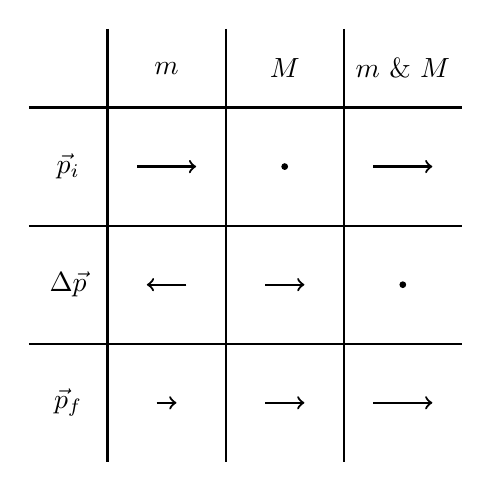
\begin{tikzpicture}
		\MVDRows{MVD}
		\MVDCol{mass}{$m$}{MVD}{0.75}
		\MVec{massinit}{0.75}
		\MVec[180]{massdelt}{0.5}
		\MVec{massfin}{0.25}
		\MVDCol{Mass}{$M$}{mass}{0.75}
		\MDot{Massinit}
		\MVec{Massdelt}{0.5}
		\MVec{Massfin}{0.5}
		\MVDCol{sys}{$m$ \& $M$}{Mass}{0.75}
		\MVec{sysinit}{0.75}
		\MDot{sysdelt}
		\MVec{sysfin}{0.75}
	\end{tikzpicture}
\end{figure}

The momentum conservation equation (choosing right as the positive direction) is
\[
mv = mv_{m} + Mv_{M}.
\]
Since the collision is perfectly elastic, we also have conservation of energy:
\[
\frac{1}{2}mv^{2} = \frac{1}{2}mv_{m}^{2} + \frac{1}{2}Mv_{M}^{2}.
\]
We can use these two equations to solve for both unknown final velocities.

First, let us simplify both expressions by dividing through by $m$ (and multiplying the energy equation by 2):
\begin{align*}
	v & = v_{m} + \frac{M}{m}v_{M}, \\
	v^{2} & = v_{m}^{2} + \frac{M}{m}v_{M}^{2}.
\end{align*}
We can write the first equation as $v_{m} = v - \frac{M}{m}v_{M}$ and substitute it into the second to get
\begin{align*}
	v^{2} & = \left(v - \frac{M}{m}v_{M}\right)^{2} + \frac{M}{m}v_{M}^{2} \\
	v^{2} & = v^{2} - 2\frac{M}{m}vv_{M} + \frac{M^{2}}{m^{2}}v_{M}^{2} + \frac{M}{m}v_{M}^{2} \\
	0 & = - 2\frac{M}{m}vv_{M} + \frac{M^{2}}{m^{2}}v_{M}^{2} + \frac{M}{m}v_{M}^{2}.
\end{align*}
Dividing through by $\frac{M}{m}v_{M}$ gives us
\begin{align*}
	0 & = - 2v + \frac{M}{m}v_{M} + v_{M} \\
	\left(1+\frac{M}{m}\right)v_{M} & = 2v \\
	v_{M} & = \frac{2m}{m+M}v.
\end{align*}
Subsituting this into our simplified momentum expression gives us
\begin{align*}
	v_{m} & = v-\frac{M}{m}\frac{2m}{m+M}v \\
	& = \left(1-\frac{2M}{m+M}\right)v \\
	& = \frac{m-M}{m+M}v.
\end{align*}
}
\Solution{\CollRockSense}{
	
\noindent\textbf{\underline{Sensemaking:}}

If $M \gg m$, then $v_{M}$ approaches zero, as predicted. We also see that $v_{m} \approx -v$, so the small rock reflects back at is original speed.

If $M = m$, then $v_{M}=v$ and $v_{m}=0$, which is the Newton's cradle behavior that we predicted.

We didn't talk about $M \ll m$, but it is interesting. In this case, $v_{m} \approx v$ (the more massive object doesn't slow down after the collision) and $v_{M} \approx 2v$ (the stationary object gets launched forward at twice the massive object's speed). In the reference frame of the massive object, the smaller object is leftbound at speed $v$ and reflects to the right at the same speed, much like the previous special case.
}
\end{document}